
\begin{frame}{Basic information}
	\textbf{The aim:} Experimental analysis of selected generalized binary search problems. The aim of the analysis is to verify the hypotheses regarding the effectiveness of search algorithms. 
    
    \textbf{Schedule:}
    \begin{itemize}
    \pause
    \item 2024.01 -- 2024.06: Researching and selection of the query model.
    \item 2024.06 -- 2025.05: Development and formal analysis of the proposed algorithms.
    \item 2025.06 -- 2025.10: Selection of models and algorithms for comparison, implementation, thesis writing.
    \item 2025.11 -- 2025.12: Execution of experiments, analysis and interpretation of the results, finalization of the thesis.

\end{itemize}
\end{frame}

\begin{frame}{State of the work}
    \begin{itemize}
        \item Implementation, about 60\% complete:
        \begin{itemize}
        \item Language: \textbf{python},
        \item Libraries: \textbf{networkx},
        \item Environment: \textbf{PyCharm},
        \item Versioning: \textbf{git} + \textbf{github}, \hyperlink{https://github.com/MSzyfel/Binary-Search}{https://github.com/MSzyfel/Binary-Search}.
        \end{itemize} 
        \pause
        \item Thesis, about 80\% complete:
        \begin{itemize}
            \item Language: \textbf{LaTeX},
            \item Environment: \textbf{Visual Studio Code},
            \item Versioning: \textbf{git} + \textbf{github}, \hyperlink{https://github.com/MSzyfel/Papers}{https://github.com/MSzyfel/Papers}.
        \end{itemize} 
        \pause
        \item What is left: 
        \begin{itemize}
            \item Experiments,
            \item Advanced data generation,
            \item Optimization,
            \item Bug fixing,
            \item Data visualization.
        \end{itemize} 
    \end{itemize}
\end{frame}
\begin{frame}{Binary Search}
    
\begin{figure}[ht]
\centering
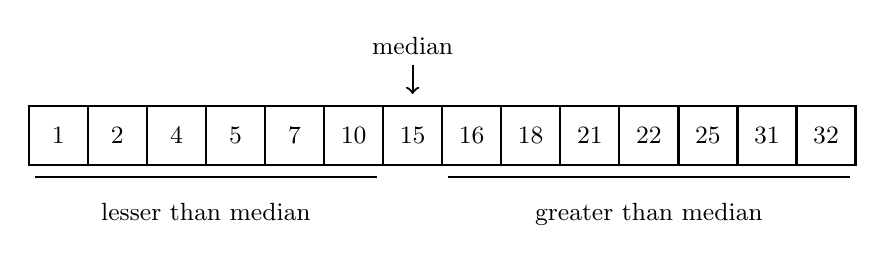
\begin{tikzpicture}[every node/.style={font=\small}, scale=0.75]

% --- Array values (10 elements) ---
\def\A{{1, 2, 4, 5, 7, 10, 15, 16, 18, 21, 22, 25, 31, 32}}
\def\MID{6} % Index of median (0-based): value = 23
% Draw array elements and indices
\foreach \i in {0,...,13} {
    \pgfmathsetmacro{\val}{\A[\i]}
    \draw[thick] (\i, 0) rectangle ++(1,1);
    \node at (\i+0.5, 0.5) {\val};
}

% Underline LEFT subarray (0..3)
\draw[thick] (0.1, -0.2) -- (6.0-0.1, -0.2);
% Label
\node[below=6pt] at (3, -0.2) {lesser than median};

% Underline RIGHT subarray (5..9)
\draw[thick] (7+0.1, -0.2) -- (13+1-0.1, -0.2);
% Label
\node[below=6pt] at (10.5, -0.2) {greater than median};

% Arrow for mid
\draw[<-, thick] (\MID+0.5, 1.2) -- +(0, 0.5) node[above] {median};

\end{tikzpicture}
\caption[Binary search]{Example of a sorted array containing 14 elements. }
\label{fig:binary-search-subarrays}
\end{figure}

\end{frame}


\begin{frame}{Generalized binary search}
        \begin{definition} A \textbf{searcher} is required to find a hidden \textbf{target} vertex $x$ in a graph $G$. To do so, they iteratively perform \textbf{queries} to an \textbf{oracle}, each about a chosen vertex $v$. After each such call, the oracle responds whether the target was found and if not, the searcher receives as a reply the connected component of $G-v$ containing the target.
        \end{definition}
	\pause

	A further generalization is to associate with each vertex a \textbf{cost} function $c:V\br{G}\to \mathbb{R}_{\geq 0}$ representing the time required to query a given vertex. 
    
\end{frame}
\begin{frame}{Example}
    \begin{figure}[htbp]
    \centering
    \begin{minipage}{0.3\textwidth}
        \centering
        \tikz [tree layout, grow=-65,
               sibling distance=11mm, level distance=13mm, scale = 0.6, thick]
          \graph {
    ""[as=$a$] -- {
        ""[as=$b$, draw=red, thick, circle] -- ""[as=$c$] -- {
            ""[as=$d$] -- ""[as=$e$],
            ""[as=$f$] -- { ""[as=$g$], ""[as=$h$], ""[as=$i$] }
        },
        ""[as=$j$] -- ""[as=$k$] -- { ""[as=$l$], ""[as=$m$] }
    }
};
    \caption{Query to $b$.}
    \end{minipage}
    \pause
    \begin{minipage}{0.3\textwidth}
        \centering
        \tikz [tree layout, grow=-65,
               sibling distance=11mm, level distance=13mm, scale = 0.6, thick]
          \graph {
        ""[as=$c$] -- {
            ""[as=$d$] -- ""[as=$e$],
            ""[as=$f$, draw=red, thick, circle] -- { ""[as=$g$], ""[as=$h$], ""[as=$i$]
        }
    }
};
    \caption{Query to $f$.}
    \end{minipage}
    
    \pause
    \begin{minipage}{0.3\textwidth}
        \centering
        \tikz [tree layout, grow=-65,
               sibling distance=11mm, level distance=13mm, scale = 0.6, thick]
          \graph {
        ""[as=$c$] -- {
            ""[as=$d$, draw=red, thick, circle] -- ""[as=$e$]
        }
};
    \caption{Query to $d$.}
    \end{minipage}
    \pause
    \begin{minipage}{0.3\textwidth}
        \centering
        \tikz [tree layout, grow=-65,
               sibling distance=11mm, level distance=13mm, scale = 0.6, thick]
          \graph {
        ""[as=$c$, draw=red, thick, circle]
};
    \caption{Query to $c$.}
    \end{minipage}
\end{figure}
\end{frame}


\begin{frame}{Classes of graphs considered}
	\textbf{There are three main classes of graphs to be considered}:
	\begin{itemize}
	\item \textbf{Paths} - equivalent to searching in a sorted array. 
    \pause
	\item \textbf{Trees} -  The most extensively studied model. \textbf{Our choice}.
    \pause
    \item \textbf{General graphs} - Computationally hardest.
	\end{itemize}
\end{frame}

\begin{frame}{Decision trees}
        \begin{definition}
        \textbf{Decision tree}:
        \begin{itemize}
            \item $D=\br{V\br{D}, E\br{D}}$, $V\br{D}=V\br{T}$ are vertices and $E\br{D}$ are edges of $D$.
            \pause
            \item $Q_D\br{T,x}$ - sequence of queries performed in order to find $x$.
            \pause
            \item \textbf{Cost} of $D$ in $\br{T,c}$:
            $$
\COST_D\br{T, c} = \max_{x\in V\br{T}} \brc{\sum_{q\in Q_{D}\br{T,x}}c\br{q}}.
$$
            \pause
        \item $\OPT\br{T, c} = \min_{D} \brc{\COST_D\br{T, c}}$ - \textbf{optimal cost}.
        \end{itemize}
        \end{definition}
\end{frame}

\begin{frame}{Example of decision tree}
    
\begin{figure}[htbp]
    \centering
    \begin{minipage}{0.34\textwidth}
        \centering
        \tikz [tree layout, grow=-65,
               sibling distance=11mm, level distance=13mm,]
          \graph {
    ""[as=$a$] -- {
        ""[as=$b$] -- ""[as=$c$] -- {
            ""[as=$d$] -- ""[as=$e$],
            ""[as=$f$] -- { ""[as=$g$], ""[as=$h$], ""[as=$i$] }
        },
        ""[as=$j$] -- ""[as=$k$] -- { ""[as=$l$], ""[as=$m$] }
    }
};
    \caption[Sample tree]{}
    \label{fig:tree}
    \end{minipage}
    \begin{minipage}{0.32\textwidth}
        \centering
        \tikz [tree layout, grow=-90,
               sibling distance=12mm, level distance=14mm,]
          \graph {
            ""[as=$c$] -> { ""[as=$j$] -> { ""[as=$a$] -> ""[as=$b$],  ""[as=$l$] -> {""[as=$k$] -> ""[as=$m$]}}, ""[as=$h$] -> {""[as=$f$] -> {""[as=$g$], ""[as=$i$]}},  ""[as=$d$] -> ""[as=$e$]}
          };
    \caption[Vertex decision tree for a tree]{}
    \label{fig:dt_t_v}
    \end{minipage}
    \begin{minipage}{0.32\textwidth}
        \centering
        \tikz [tree layout, grow=-90,
               sibling distance=12mm, level distance=14mm,]
            \graph {
              ""[as=$aj$] -> {
                ""[as=$cf$] -> {""[as=$cd$] -> {""[as=$bc$], ""[as=$de$]},  ""[as=$fg$] -> ""[as=$fh$] -> ""[as=$fi$]]},
                ""[as=$km$] -> ""[as=$jk$] -> ""[as=$kl$]
              }
            };
        \caption[Edge decision tree for a tree]{}
        \label{fig:dt_t_e}
    \end{minipage}
        \caption[Tree and decision trees for it]{Sample input tree $T$ (Figure \ref{fig:tree}) and two decision trees for $T$: one for the Vertex Tree Search Problem (Figure \ref{fig:dt_t_v}) and one for the Edge Tree Search Problem (Figure \ref{fig:dt_t_e}).}
        \label{fig:sample_decision_trees_for_tree}
\end{figure}
\end{frame}

\begin{frame}{Problem statement}

    \begin{definition}
        Given a tree $T$ and weight function $c$, the \textbf{Tree Search Problem} consists of finding a decision tree $D$, such that $\COST_D\br{T,c}=\OPT\br{T,c}$.
    \end{definition}

    \pause

    Unluckily, the Tree Search Problem is \textbf{strongly NP-Hard} even when restricted to binary trees and spiders of diameter at most 6. However, one can find \textbf{approximate} solutions. 

\end{frame}
